\section{1174035 Luthfi Muhammad Nabil}

\subsection{Teori}
\begin{enumerate}
\item Jelaskan Apa Itu Binary Classification dilengkapi ilustrasi gambar sendiri.\par
Binary Classification adalah sebuah metode untuk menklasifikasikan elemen yang dibentuk seperti grup untuk dibagi menjadi 2 grup. Dari 2 grup tersebut diprediksikan setiap anggota pada grup yang mana sesuai dengan yang diatur pada aturan klasifikasi. Data atau konteks yang didapat membutuhkan keputusan dari item tersebut memiliki properti kualitatif, karakteristik yang spesifik, atau tipikal klasifikasi biner.
\begin{figure}[H]
\centering
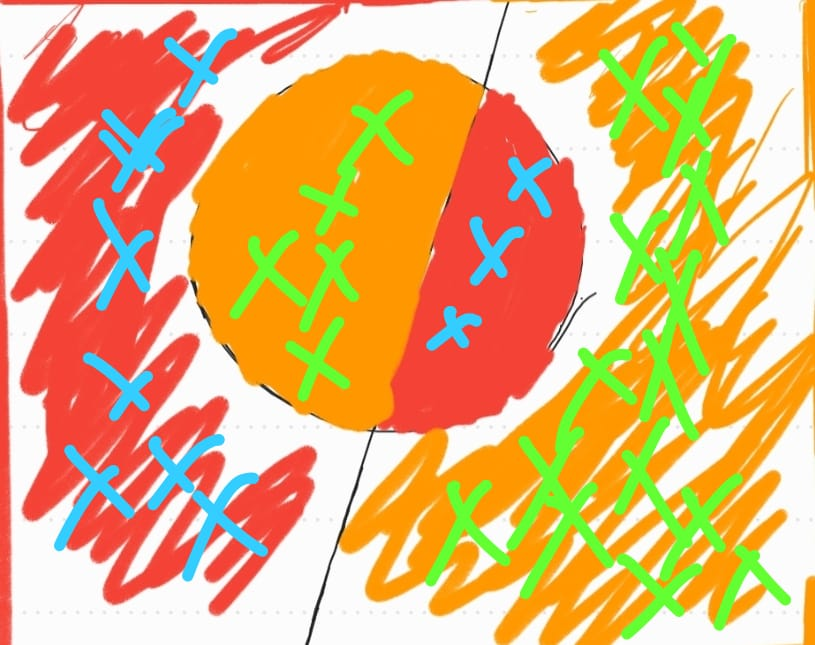
\includegraphics[scale=0.2]{figures/1174035/chapter2/binary_classification.jpeg}
\caption{contoh binary classification}
\label{contoh}
\end{figure}


\item Jelaskan Apa itu supervised learning , unsupervised learning dan clusterring dengan ilustrasi gambar sendiri.\par
Supervised learning adalah kondisi yang menggunakan variabel input dan output untuk dapat dilakukan pemetaan input output yang sudah didapat. Disebud Supervised Learning karena proses dari pembelajaran algoritma dari pembelajan yang disumberkan dengan dataset dapat dipikirkan seperti seorang guru yang mengawasi proses pembelajaran. Proses pembelajaran dari algoritma akan berhenti saat algoritma sudah mendapatkan level dari performansi yang dapat diterima. \par
Unsupervised learning adalah kondisi dimana kamu hanya memiliki input data tanpa memiliki variabel output yang sesuai. Tujuan dari unsupervised learning adalah untuk memodelkan distribusi pada data untuk mengetahui lebih lanjut mengenai data. Disebut unsupervised learning karena pada metode ini, tidak ada jawaban yang tepat dan tidak ada pengarah. Sehingga algoritma akan ditinggalkan sesuai rancangan demi menemukan dan dapat mengolah data yang menarik pada saat yang akan datang. \par
Clustering adalah sebuah metode untuk membedakan data - data menjadi kumpulan dari group yang isinya merupakan data yang serupa setiap grupnya. Basisnya dapat berupa kesamaan atau perbedaan dari setiap grup tersebut. \par
\begin{figure}[H]
\centering
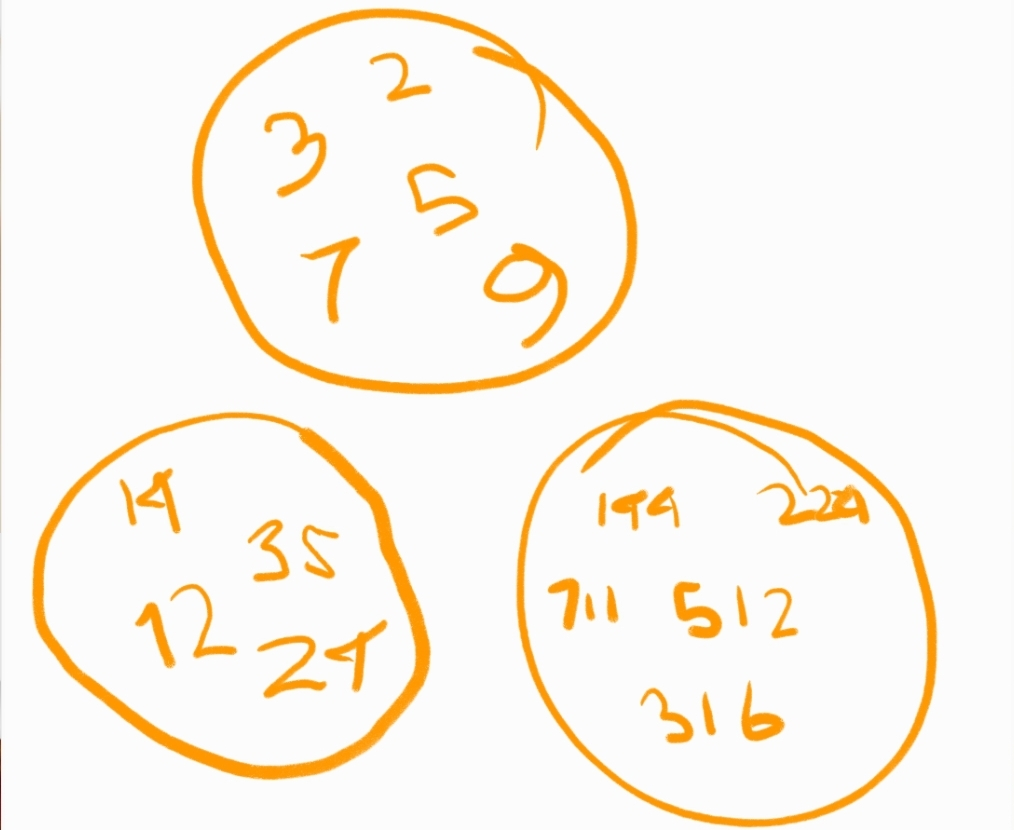
\includegraphics[scale=0.2]{figures/1174035/chapter2/clustering.jpeg}
\caption{contoh clustering}
\label{contoh}
\end{figure}


\item Jelaskan apa itu evaluasi dan akurasi dan disertai ilustrasi contoh dengan gambar sendiri.\par
Evaluasi adalah kegiatan yang dilakukan untuk menentukan sebuah nilai yang dapat diambil dari suatu hal. Beberapa contoh evaluasi diantaranya menilai sebuah barang, bahaya dari penyakit, dan lain sebagainya dengan parameter yang digunakan yaitu mengetahui faktor - faktor yang menyebabkan atau akibat yang akan terjadi jika dibiarkan. 

\item Jelaskan bagaimana cara membuat Confusion Matrix, Buat confusion matrix sendiri.\par
Confusion Matrix merupakan metode untuk menghitung akurasi pada data mining atau Sistem Pendukung Keputusan. Untuk menggunakan Confusion Matrix, ada 4 istilah sebagai hasil proses dari klasifikasi. Diantaranya adalah :

\begin{itemize}
    \item True Positive : Data positif yang terdeteksi memiliki hasil benar
    \item False Positive : Data Positif yang terdeteksi memiliki hasil salah
    \item True Negative : Data negatif yang terdeteksi memiliki hasil benar
    \item False Negative : Data negatif yang terdeteksi memiliki hasil salah
\end{itemize}


\item Jelaskan bagaimana K-fold cross validation bekerja dengan gambar ilustrasi contoh buatan sendiri.
k-Fold Cross-Validation merupakan prosedur untuk mengambil sampel ulang yang digunakan untuk mengevaluasi sebuah "machine learning" model pada sampel data yang terbatas. Procedure yang ada memiliki satu parameter yang dipanggil k yang mengacu pada jumlah grup yang memberikan data sampel untuk dipisahkan.
K-fold Cross-validation akan melakukan hal berikut : 
\begin{enumerate}
    \item Mengacak dataset secara random
    \item Memisahkan dataset menjadi k group
    \item Untuk setiap grup, akan disesuaikan dan dievaluasikan
    \item Merekaphasil dari evaluasi dan penyesuaian menggunakan sampel dari model evaluasi
\end{enumerate}
\begin{figure}[H]
\centering
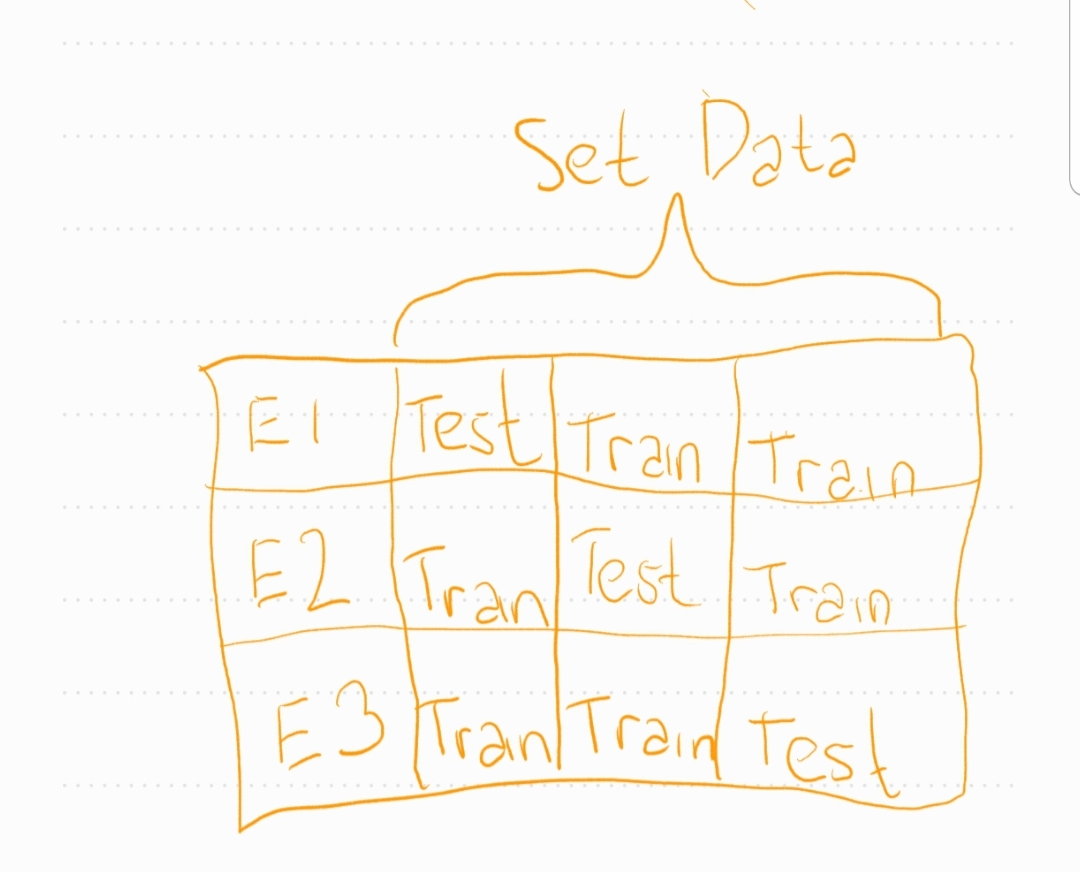
\includegraphics[scale=0.2]{figures/1174035/chapter2/kcode.jpeg}
\caption{contoh K-fold cross validation}
\label{contoh}
\end{figure}


\item Jelaskan Apa itu decision tree disertakan gambar ilustrasi contoh buatan sendiri.\par
Decision Tree merupakan sebuah struktur yang menentukan keputusan dan setiap konsekuensinya. Hasil dari setiap struktur biasanya menggunakan jawaban (True dan False) atau cabang lain yang akan menjadi pohon selanjutnya. Setiap keputusan diantaranya akan membandingkan kondisi yang diberikan kepada struktur untuk dibandingkan kondisi apa saja yang sudah didapat pada sistem tersebut. 


\item jelaskan apa itu information gain dan entropi dengan gambar ilustrasi buatan sendiri.\par
Information Gain merupakan total data yang didapat dari data - data acak yang data tersebut akan digunakan untuk analisis data lainnya. Information Gain ini digunakan pada decision tree sebagai label setiap aksi - aksi yang perlu dinilai validasinya. 
\begin{figure}[H]
\centering
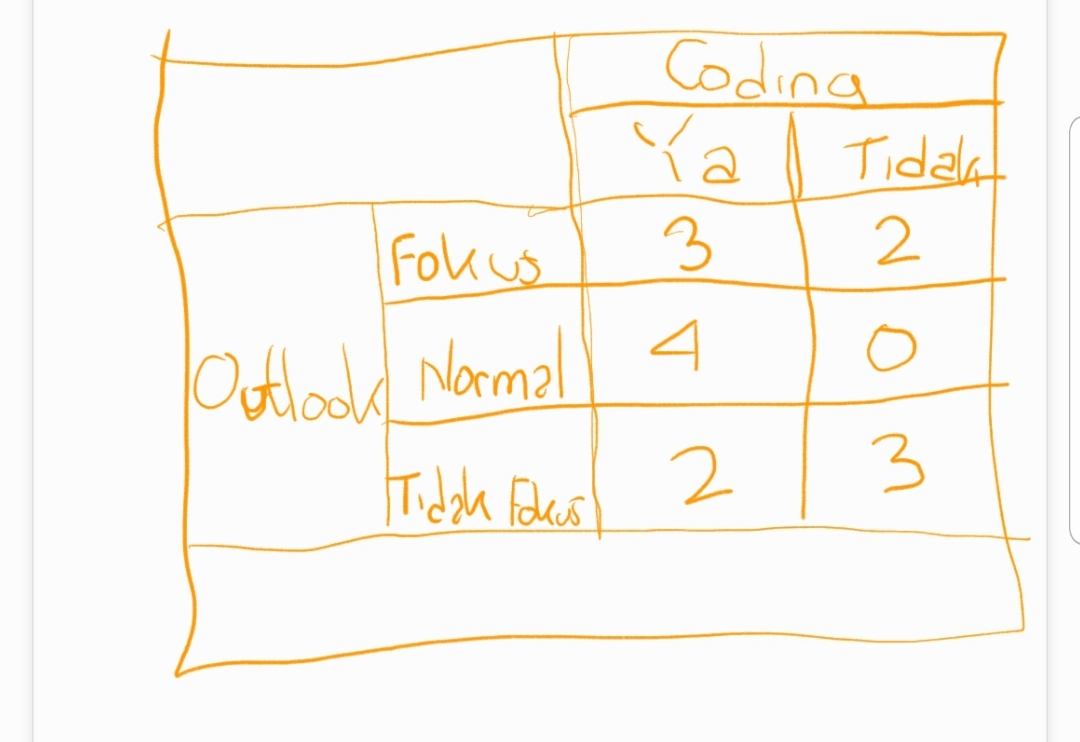
\includegraphics[scale=0.2]{figures/1174035/chapter2/info_gain.jpeg}
\caption{contoh information gain}
\label{contoh}
\end{figure}
Entropi merupakan pengukuran sebuah data dan validnya data tersebut untuk dapat digunakan sebagai informasi yang akan dimasukkan ke Information Gain. Entropi menilai sebuah obyek berdasarkan kebutuhan di dunia nyata dan pengaruh pada sistem yang akan digunakan
\begin{figure}[H]
    \centering
    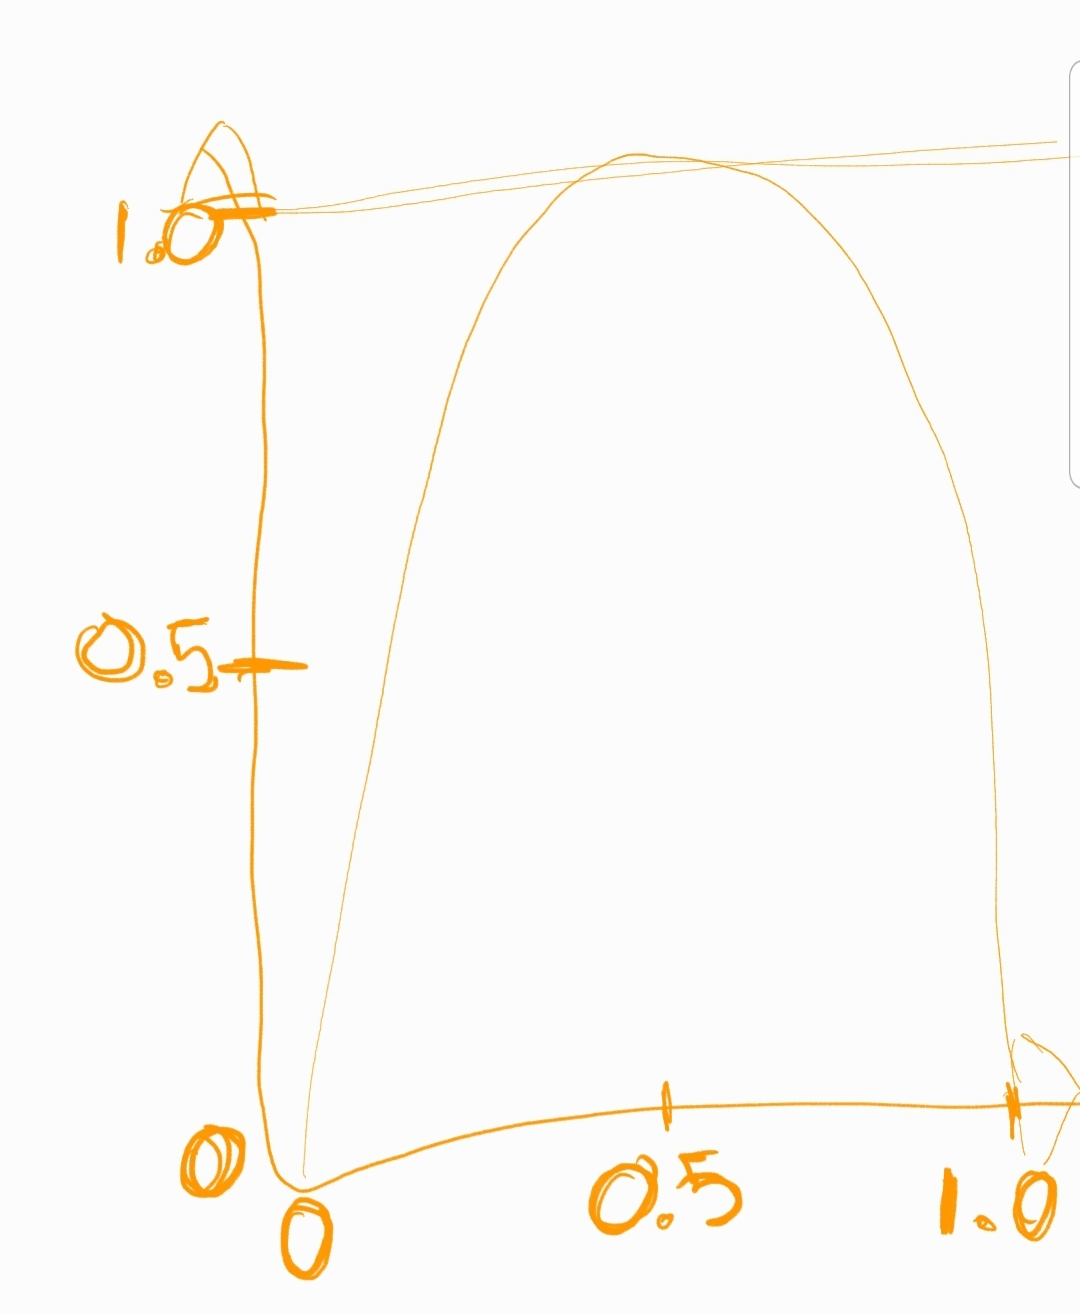
\includegraphics[scale=0.2]{figures/1174035/chapter2/entropi.jpeg}
    \caption{contoh information gain}
    \label{contoh}
    \end{figure}
\end{enumerate}

\subsection{Scikit-Learn}
\begin{enumerate}
    \item \hfill \break \lstinputlisting[firstline=11, lastline=13]{src/1174035/chapter2/sample1.py}
	\begin{figure}[H]
		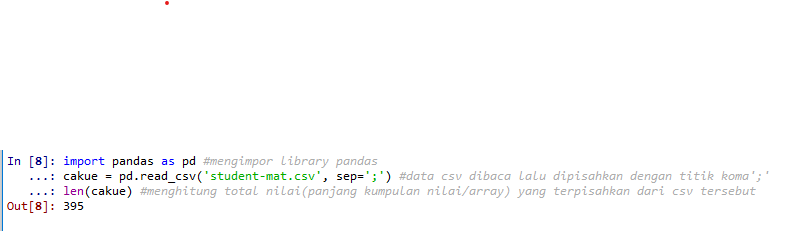
\includegraphics[width=4cm]{figures/1174035/chapter2/1.png}
		\centering
		\caption{Hasil Percobaan 1}
    \end{figure}
    \item \hfill \break \lstinputlisting[firstline=15, lastline=17]{src/1174035/chapter2/sample1.py}
	\begin{figure}[H]
		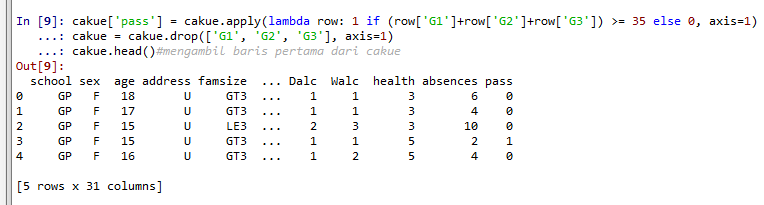
\includegraphics[width=4cm]{figures/1174035/chapter2/2.png}
		\centering
		\caption{Hasil Percobaan 2}
    \end{figure}
    \item \hfill \break \lstinputlisting[firstline=19, lastline=20]{src/1174035/chapter2/sample1.py}
	\begin{figure}[H]
		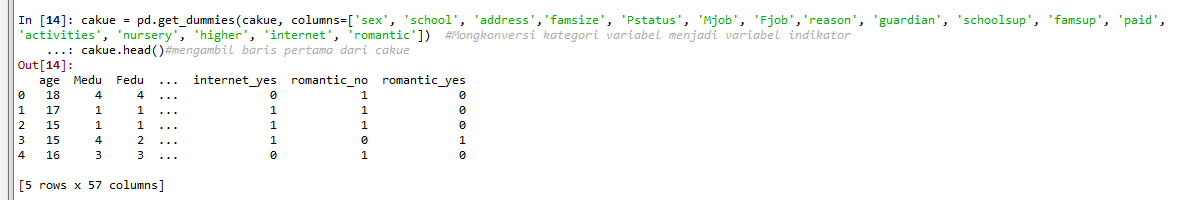
\includegraphics[width=4cm]{figures/1174035/chapter2/3.png}
		\centering
		\caption{Hasil Percobaan 3}
    \end{figure}
    \item \hfill \break \lstinputlisting[firstline=22, lastline=35]{src/1174035/chapter2/sample1.py}
	\begin{figure}[H]
		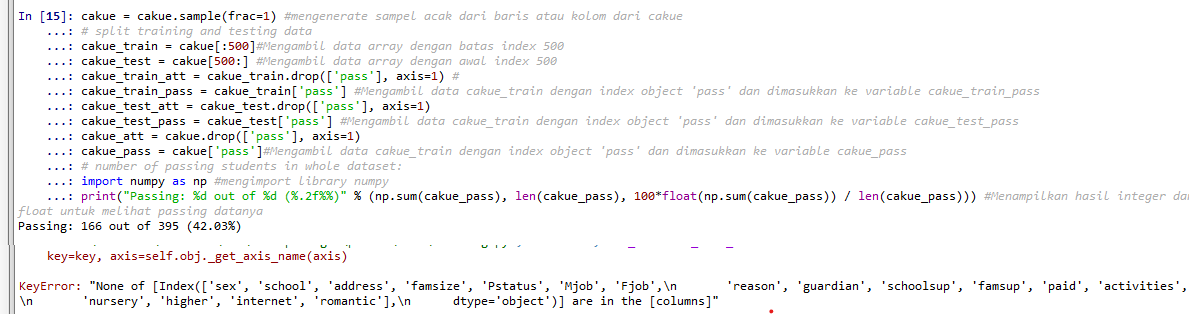
\includegraphics[width=4cm]{figures/1174035/chapter2/4.png}
		\centering
		\caption{Hasil Percobaan 4}
    \end{figure}
    \item \hfill \break \lstinputlisting[firstline=37, lastline=39]{src/1174035/chapter2/sample1.py}
	\begin{figure}[H]
		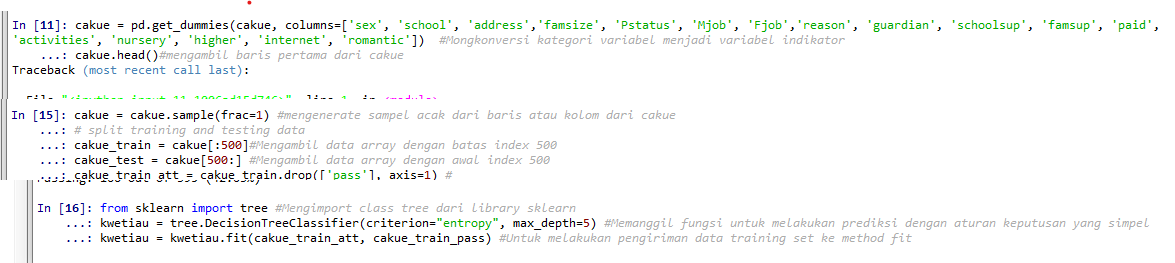
\includegraphics[width=4cm]{figures/1174035/chapter2/5.png}
		\centering
		\caption{Hasil Percobaan 5}
    \end{figure}
    \item \hfill \break \lstinputlisting[firstline=41, lastline=44]{src/1174035/chapter2/sample1.py}
	\begin{figure}[H]
		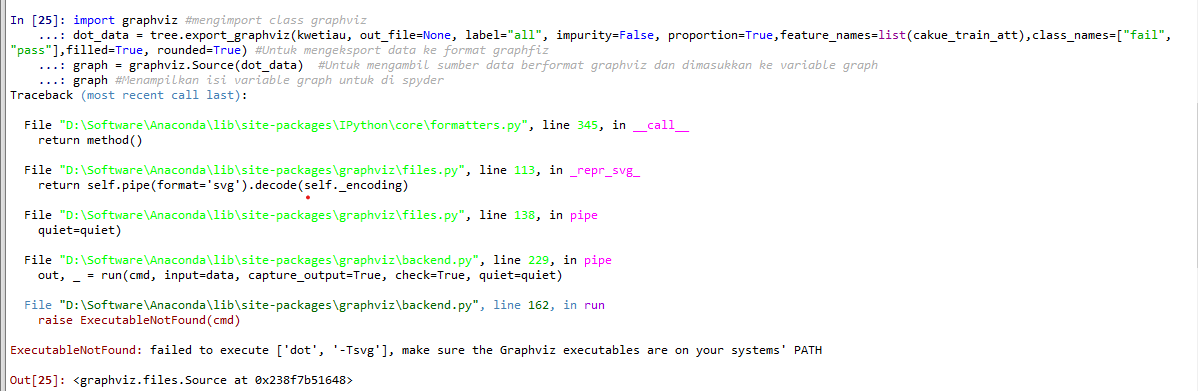
\includegraphics[width=4cm]{figures/1174035/chapter2/6.png}
		\centering
		\caption{Hasil Percobaan 6}
    \end{figure}
    \item \hfill \break \lstinputlisting[firstline=46, lastline=46]{src/1174035/chapter2/sample1.py}
	\begin{figure}[H]
		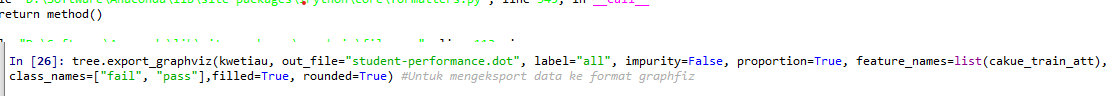
\includegraphics[width=4cm]{figures/1174035/chapter2/7.png}
		\centering
		\caption{Hasil Percobaan 7}
    \end{figure}
    \item \hfill \break \lstinputlisting[firstline=48, lastline=48]{src/1174035/chapter2/sample1.py}
	\begin{figure}[H]
		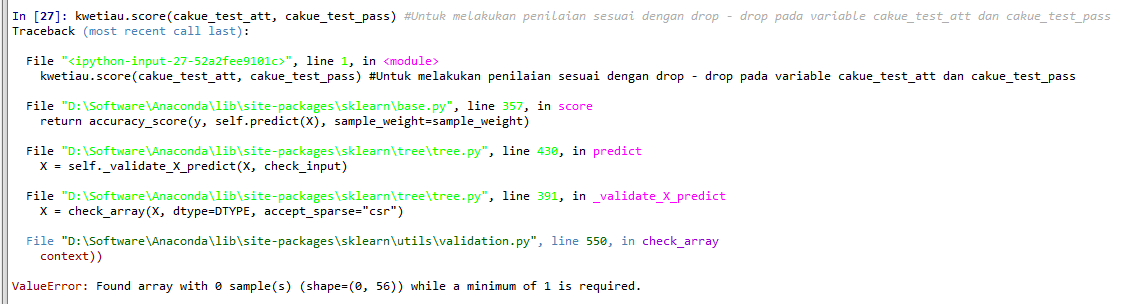
\includegraphics[width=4cm]{figures/1174035/chapter2/8.png}
		\centering
		\caption{Hasil Percobaan 8}
    \end{figure}
    \item \hfill \break \lstinputlisting[firstline=50, lastline=54]{src/1174035/chapter2/sample1.py}
	\begin{figure}[H]
		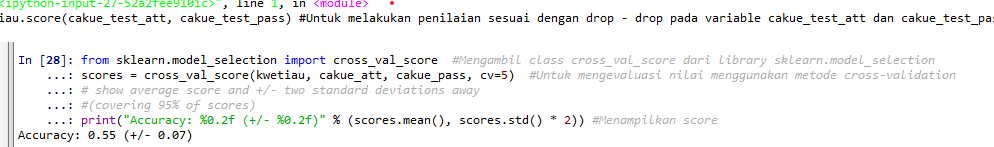
\includegraphics[width=4cm]{figures/1174035/chapter2/9.png}
		\centering
		\caption{Hasil Percobaan 9}
    \end{figure}
    \item \hfill \break \lstinputlisting[firstline=56, lastline=59]{src/1174035/chapter2/sample1.py}
	\begin{figure}[H]
		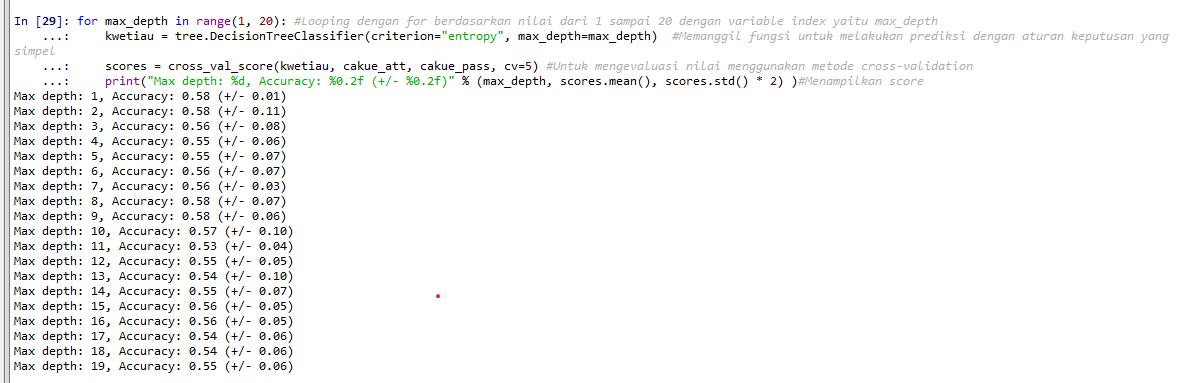
\includegraphics[width=4cm]{figures/1174035/chapter2/10.png}
		\centering
		\caption{Hasil Percobaan 10}
    \end{figure}
    \item \hfill \break \lstinputlisting[firstline=61, lastline=70]{src/1174035/chapter2/sample1.py}
	\begin{figure}[H]
		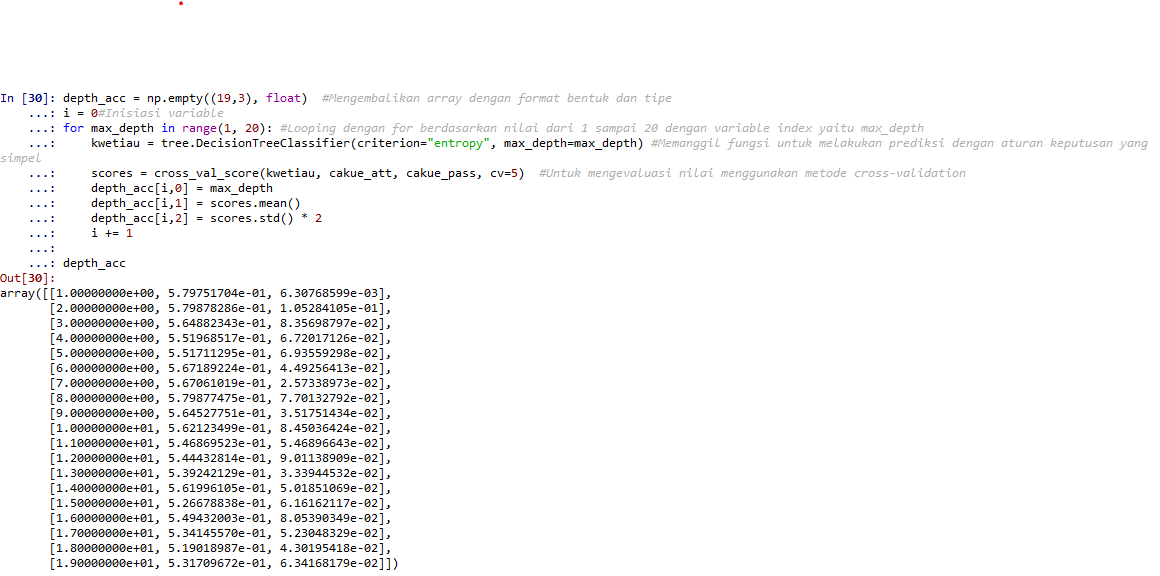
\includegraphics[width=4cm]{figures/1174035/chapter2/11.png}
		\centering
		\caption{Hasil Percobaan 11}
    \end{figure}
    \item \hfill \break \lstinputlisting[firstline=72, lastline=75]{src/1174035/chapter2/sample1.py}
	\begin{figure}[H]
		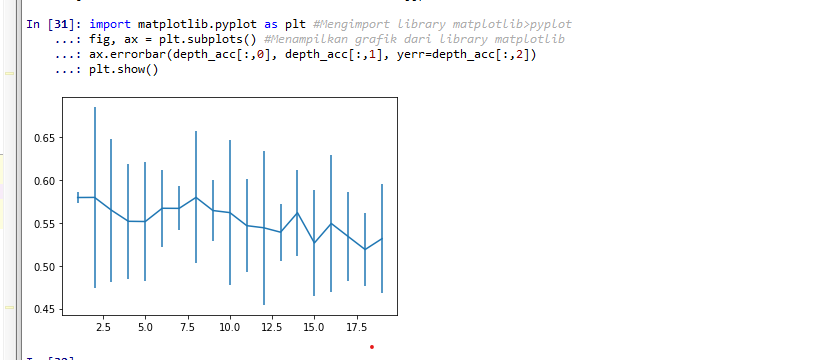
\includegraphics[width=4cm]{figures/1174035/chapter2/12.png}
		\centering
		\caption{Hasil Percobaan 12}
	\end{figure}
\end{enumerate}
\subsection{Skrinsut Error}
Error yang didapat yaitu mengalami error tidak ada library graphviz yang terdeteksi
\begin{figure}[H]
    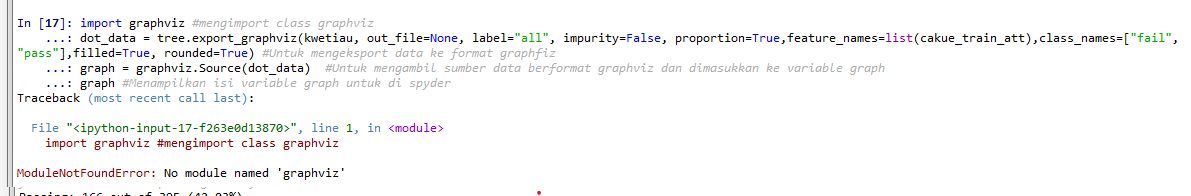
\includegraphics[width=4cm]{figures/1174035/chapter2/error.png}
    \centering
    \caption{Error}
\end{figure}
\subsection{Penanganan Error}
Solusinya adalah dengan menginstall library graphviz yang ada
\begin{figure}[H]
    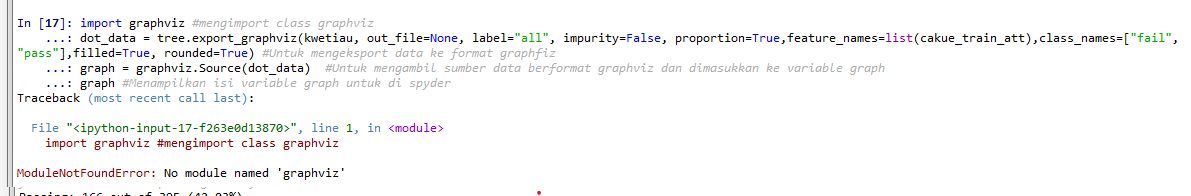
\includegraphics[width=4cm]{figures/1174035/chapter2/error.png}
    \centering
    \caption{Error}
\end{figure}
\subsection{Plagiarisme}
\begin{figure}[H]
    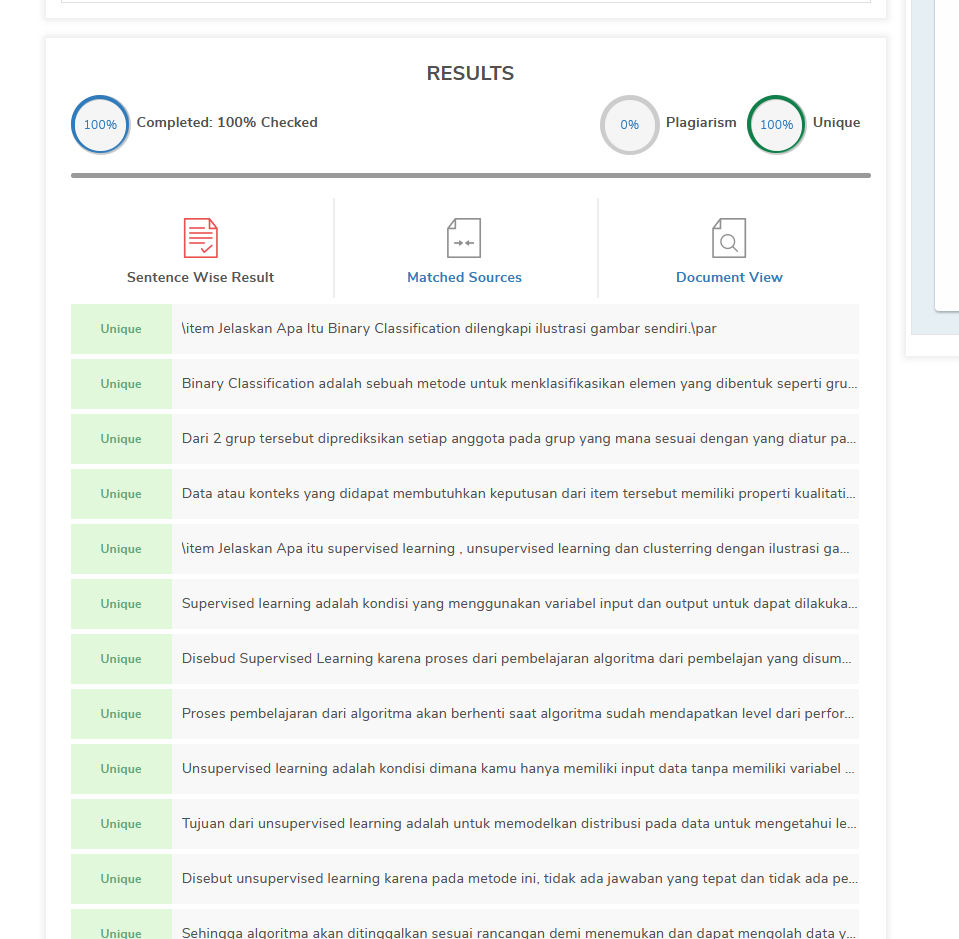
\includegraphics[width=4cm]{figures/1174035/chapter2/plagiarism.png}
    \centering
    \caption{Hasil Pengecekan Plagiarisme}
\end{figure}
